\chapter{Arhitektura i dizajn sustava}

\textbf{\textit{dio 1. revizije}}\\

\section*{Uvod u Arhitekturu Sustava}
Naš sustav je dizajniran da bude efikasan, skalabilan i pouzdan. U nastavku detaljno opisujemo arhitekturu našeg sustava.

\subsection*{Izbor Arhitekture}
\begin{itemize}
    \item Naša odluka da koristimo trodjelnu arhitekturu temelji se na principima oblikovanja predstavljenim na predavanjima, gdje se ističe važnost modularnosti i odvajanja odgovornosti. Ovaj pristup omogućava bolje upravljanje kompleksnošću sustava i lakše održavanje.
\end{itemize}

\subsection*{Organizacija Sustava}
\begin{itemize}
    \item Sustav je organiziran na visokoj razini apstrakcije, koristeći klijent-poslužitelj model, što omogućuje razdvajanje korisničkog sučelja od poslovne logike.
\end{itemize}

\subsection*{Detalji Podsustava}
\subsubsection*{Backend (Spring Boot)}
\begin{itemize}
    \item Backend služi kao osnova našeg sustava, sadrži više podsustava kao što su servisi i kontroleri koji obrađuju poslovne zahtjeve.
    \item Komunikacija s bazom podataka vrši se kroz PostgreSQL, što omogućava efikasnu organizaciju i manipulaciju podacima.
\end{itemize}

\subsubsection*{Frontend (Node.js i JavaScript)}
\begin{itemize}
    \item Frontend je organiziran u komponente i kontejnere, pružajući fleksibilno i intuitivno korisničko sučelje.
    \item REST API se koristi za komunikaciju s backendom, što osigurava brzu i pouzdanu razmjenu podataka.
\end{itemize}

\subsubsection*{Baza podataka (PostgreSQL)}
\begin{itemize}
    \item Centralno spremište za sve relevantne podatke sustava, omogućuje pouzdanu pohranu i pristup podacima.
    \item Struktura baze je dizajnirana da podržava složene upite i relacije između različitih podataka.
\end{itemize}

\subsection*{Mrežni Protokoli i Komunikacija}
\begin{itemize}
    \item Komunikacija između klijenta i poslužitelja odvija se preko HTTP/HTTPS protokola, osiguravajući sigurnost i standardiziran protok informacija.
\end{itemize}

\subsection*{Globalni Upravljački Tok}
\begin{itemize}
    \item Globalni upravljački tok je definiran kroz MVC arhitekturu, gdje Model upravlja podacima, View prikazuje podatke, a Controller upravlja interakcijom korisnika s aplikacijom.
\end{itemize}

\subsection*{Sklopovsko-Programski Zahtjevi}
\begin{itemize}
    \item Sustav je prilagođen za rad na modernim računalnim platformama, uzimajući u obzir potrebe za visokom dostupnošću i performansama.
\end{itemize}

\subsection*{Skice Arhitekture}
\textit{[Ovdje dodajte skice arhitekture koje ilustriraju organizaciju sustava, MVC arhitekturu, i podsustave.]}

		\section{Baza podataka}
			
			\textbf{\textit{dio 1. revizije}}\\
			
Koristili smo PostgreSQL relacijsku bazu podataka. PostgreSQL je snažan i visoko prilagodljiv sustav za upravljanje bazama podataka, što ga čini prikladnim izborom za učinkovito i sigurno upravljanje zdravstvenim podacima, osiguravajući da su informacije o pacijentima, terminima, zdravstvenom osoblju i opremi sigurno pohranjene i dostupne. 
Svaka tablica ima primarni ključ koji jedinstveno identificira zapise unutar tablice. Baza podataka uspostavlja odnose između tablica koristeći strane ključeve. Ograničenja su postavljena kako bi se očuvao integritet podataka.  
		
			\subsection{Opis tablica}
			

				\textit{Svaku tablicu je potrebno opisati po zadanom predlošku. Lijevo se nalazi točno ime varijable u bazi podataka, u sredini se nalazi tip podataka, a desno se nalazi opis varijable. Svjetlozelenom bojom označite primarni ključ. Svjetlo plavom označite strani ključ}
				
\textbf{\_User } Ovaj entitet predstavlja korisnike sustava s različitim ulogama.  Sadrži atribute kao što su status korisnika (active), jedinstveni identifikator (id), e-mail adresa (email), ime (first\_name), prezime (last\_name), lozinka (password) i uloga korisnika (role). Provjerava se uloga korisnika kroz ograničenje \_user\_role\_check. Ovaj entitet omogućuje upravljanje korisnicima sustava i dodjeljivanje uloga kako bi se pristup određenim funkcionalnostima kontrolirao.  Primarni ključ (\_user\_pkey) je definiran na atributu id. 

\begin{longtblr}[
    label=none,
    entry=none
]{
    width = \textwidth,
    colspec={|X[6,l]|X[6, l]|X[20, l]|}, 
    rowhead = 1,
}
\hline \SetCell[c=3]{c}{\textbf{ \_user}} \\ \hline[3pt]
\SetCell{LightGreen}id & BIGINT & Jedinstveni identifikator korisnika \\ \hline
active & BOOLEAN & Označava je li korisnik aktivan \\ \hline 
email & VARCHAR & E-mail adresa korisnika \\ \hline 
first\_name & VARCHAR & Ime korisnika \\ \hline 
last\_name & VARCHAR & Prezime korisnika \\ \hline 
password & VARCHAR & Lozinka korisnika \\ \hline 
role & VARCHAR & Rola korisnika (mora biti jedna od predefiniranih uloga) \\ \hline 
\end{longtblr}

				
		
\textbf{Imenik} Entitet koji služi za pohranu informacija o osobama. Sadrži atribute kao što su jedinstveni identifikator osobe (hlkid), ime (first\_name), prezime (last\_name), specijalizacija i informacija o aktivnosti osobe.  Primarni ključ (Imenik\_pkey) je definiran na atributu hlkid. 
\begin{longtblr}[
    label=none,
    entry=none
]{
    width = \textwidth,
    colspec={|X[6,l]|X[6, l]|X[20, l]|}, 
    rowhead = 1,
}
\hline \SetCell[c=3]{c}{\textbf{imenik}} \\ \hline[3pt]
\SetCell{LightGreen}hlkid & VARCHAR & Jedinstveni identifikator imenika \\ \hline
first\_name & VARCHAR & Ime osobe \\ \hline 
last\_name & VARCHAR & Prezime osobe  \\ \hline 
specialization & VARCHAR & Stručnost osobe  \\ \hline 
active & BOOLEAN & Označava je li osoba u imeniku aktivna \\ \hline 
\end{longtblr}


\textbf{Appointment} Čuva informacije o terminima unutar sustava. Sadrži atribute kao što su datum i vrijeme termina (date\_time), identifikator zaposlenika (employee\_id), jedinstveni identifikator termina (id), identifikator pacijenta (patient\_id), identifikator sesije (session\_id), identifikator terapije (therapy\_id) i status termina. Ovaj entitet je povezan s drugim entitetima(employee, patient , session, therapy) putem različitih Many-to-One veza prema atributima \verb|employee_id|, \verb|patient_id|, \verb|session_id|, i \verb|therapy_id|. 

\begin{longtblr}[
    label=none,
    entry=none
]{
    width = \textwidth,
    colspec={|X[6,l]|X[6, l]|X[20, l]|}, 
    rowhead = 1,
}
\hline \SetCell[c=3]{c}{\textbf{appointment}} \\ \hline[3pt]
\SetCell{LightGreen}id & BIGINT & Jedinstveni identifikator termina \\ \hline 
date\_time & TIMESTAMP & Datum i vrijeme termina \\ \hline
\SetCell{LightBlue}employee\_id & BIGINT & Identifikator zaposlenika koji obavlja termin \\ \hline 
\SetCell{LightBlue}patient\_id & BIGINT & Identifikator pacijenta koji ima termin \\ \hline 
\SetCell{LightBlue}session\_id & BIGINT & Identifikator sesije kojoj pripada termin \\ \hline 
\SetCell{LightBlue}therapy\_id & BIGINT & Identifikator terapije koja se izvodi tijekom termina \\ \hline 
status & VARCHAR & Status termina \\ \hline 
\end{longtblr}

\textbf{Employee} Ovaj entitet predstavlja tablicu koja sadrži informacije o zaposlenicima. Sadrži atribute kao što su specijalizacija (specialization) i identifikator (id).
Ograničenje employee\_specialization\_check provjerava ispravnost specijalizacije. Primarni ključ (employee\_pkey) je definiran na atributu id. Povezan je One-to-Many vezom s entitetom session preko atributa employee\_id.
\end{itemize}
 
\begin{longtblr}[
    label=none,
    entry=none
]{
    width = \textwidth,
    colspec={|X[6,l]|X[6, l]|X[20, l]|}, 
    rowhead = 1,
}
\hline \SetCell[c=3]{c}{\textbf{employee}} \\ \hline[3pt]
\SetCell{LightGreen}id & BIGINT & Jedinstveni identifikator zaposlenika \\ \hline 
specialization & SMALLINT & Stručnost zaposlenika \\ \hline

\end{longtblr}

\textbf{Equipment} Ovaj entitet predstavlja tablicu equipment koja sadrži informacije o opremi.
\begin{longtblr}[
    label=none,
    entry=none
]{
    width = \textwidth,
    colspec={|X[6,l]|X[6, l]|X[20, l]|}, 
    rowhead = 1,
}
\hline \SetCell[c=3]{c}{\textbf{equipment}} \\ \hline[3pt]
\SetCell{LightGreen}id & BIGINT & Jedinstveni identifikator opreme \\ \hline 
capacity & INTEGER & Kapacitet opreme \\ \hline
description & VARCHAR & Opis opreme \\ \hline 
name & VARCHAR & Naziv opreme \\ \hline 
\end{longtblr}

\textbf{Patient} Ovaj entitet predstavlja tablicu  koja sadrži informacije o pacijentima.  Sadrži atribute kao što su datum rođenja, identifikator (id), adresa, MBO (matični broj osiguranika) i broj telefona. Primarni ključ (patient\_pkey) je definiran na atributu id.
 
\begin{longtblr}[
    label=none,
    entry=none
]{
    width = \textwidth,
    colspec={|X[6,l]|X[6, l]|X[20, l]|}, 
    rowhead = 1,
}
\hline \SetCell[c=3]{c}{\textbf{patient}} \\ \hline[3pt]
\SetCell{LightGreen}id & BIGINT & Jedinstveni identifikator pacijenta \\ \hline 
date \_of\_birth & DATE & Datum rođenja pacijenta \\ \hline
address & VARCHAR & Adresa pacijenta \\ \hline 
mbo & VARCHAR & Matični broj osiguranika pacijenta \\ \hline 
phone\_number & VARCHAR & Broj telefona pacijenta \\ \hline 
\end{longtblr}

\textbf{Session} Ovaj entitet predstavlja tablicu koja sadrži informacije o sesijama.  Sadrži atribute kao što su datum i vrijeme, identifikator zaposlenika, identifikator sesije i povratna informacija (feedback). Primarni ključ (session\_pkey) je definiran na atributu id. Povezan je Many-to-One vezom s entitetom employee preko atributa employee\_id. 
\begin{longtblr}[
    label=none,
    entry=none
]{
    width = \textwidth,
    colspec={|X[6,l]|X[6, l]|X[20, l]|}, 
    rowhead = 1,
}
\hline \SetCell[c=3]{c}{\textbf{session}} \\ \hline[3pt]
\SetCell{LightGreen}id & BIGINT & Jedinstveni identifikator sesije \\ \hline
date\_time & timestamp & Vrijeme sesije \\ \hline 
\SetCell{LightBlue}employee\_id & BIGINT & Identifikator zaposlenika \\ \hline 
feedback & character varying(255) & Povratna informacija o sesiji \\ \hline 
\end{longtblr}


\textbf{Therapy}  Ovaj entitet predstavlja tablicu koja sadrži informacije o terapijama.  Sadrži atribut identifikator (id) i atribut therapy\_type\_id. Primarni ključ (therapy\_pkey) je definiran na atributu id.  Također sadrži jedinstveno ograničenje therapy\_therapy\_type\_id\_key na atributu therapy\_type\_id. Povezan je One-to-One vezom s entitetom appointment preko atributa therapy\_id.
\begin{longtblr}[
    label=none,
    entry=none
]{
    width = \textwidth,
    colspec={|X[6,l]|X[6, l]|X[20, l]|}, 
    rowhead = 1,
}
\hline \SetCell[c=3]{c}{\textbf{therapy}} \\ \hline[3pt]
\SetCell{LightGreen}id & BIGINT & Jedinstveni identifikator terapije \\ \hline
\SetCell{LightBlue}therapy\_type\_id & BIGINT & Identifikator vrste terapije \\ \hline 
\end{longtblr}

\textbf{Therapy\_type} Ovaj entitet predstavlja tablicu koja sadrži informacije o vrstama terapija. - Sadrži atribute kao što su identifikator (id), identifikator potrebne opreme (required\_equipment\_id) i opis.  Primarni ključ (therapy\_type\_pkey) je definiran na atributu id. - Povezan je Many-to-One vezom s entitetom therapy preko atributa required\_equipment\_id i s entitetom equipment preko atributa required\_equipment\_id. 
\begin{longtblr}[
    label=none,
    entry=none
]{
    width = \textwidth,
    colspec={|X[6,l]|X[6, l]|X[20, l]|}, 
    rowhead = 1,
}
\hline \SetCell[c=3]{c}{\textbf{therapy\_type}} \\ \hline[3pt]
\SetCell{LightGreen}id & BIGINT & Jedinstveni identifikator vrste terapije \\ \hline
\SetCell{LightBlue}required\_equipment\_id & BIGINT & Identifikator potrebnog opreme \\ \hline 
description & character varying(255) & Opis vrste terapije \\ \hline 
\end{longtblr}





				
				
			
			\subsection{Dijagram baze podataka}
				\textit{ U ovom potpoglavlju potrebno je umetnuti dijagram baze podataka. Primarni i strani ključevi moraju biti označeni, a tablice povezane. Bazu podataka je potrebno normalizirati. Podsjetite se kolegija "Baze podataka".}
			\begin{figure}[h]
			    \centering
			    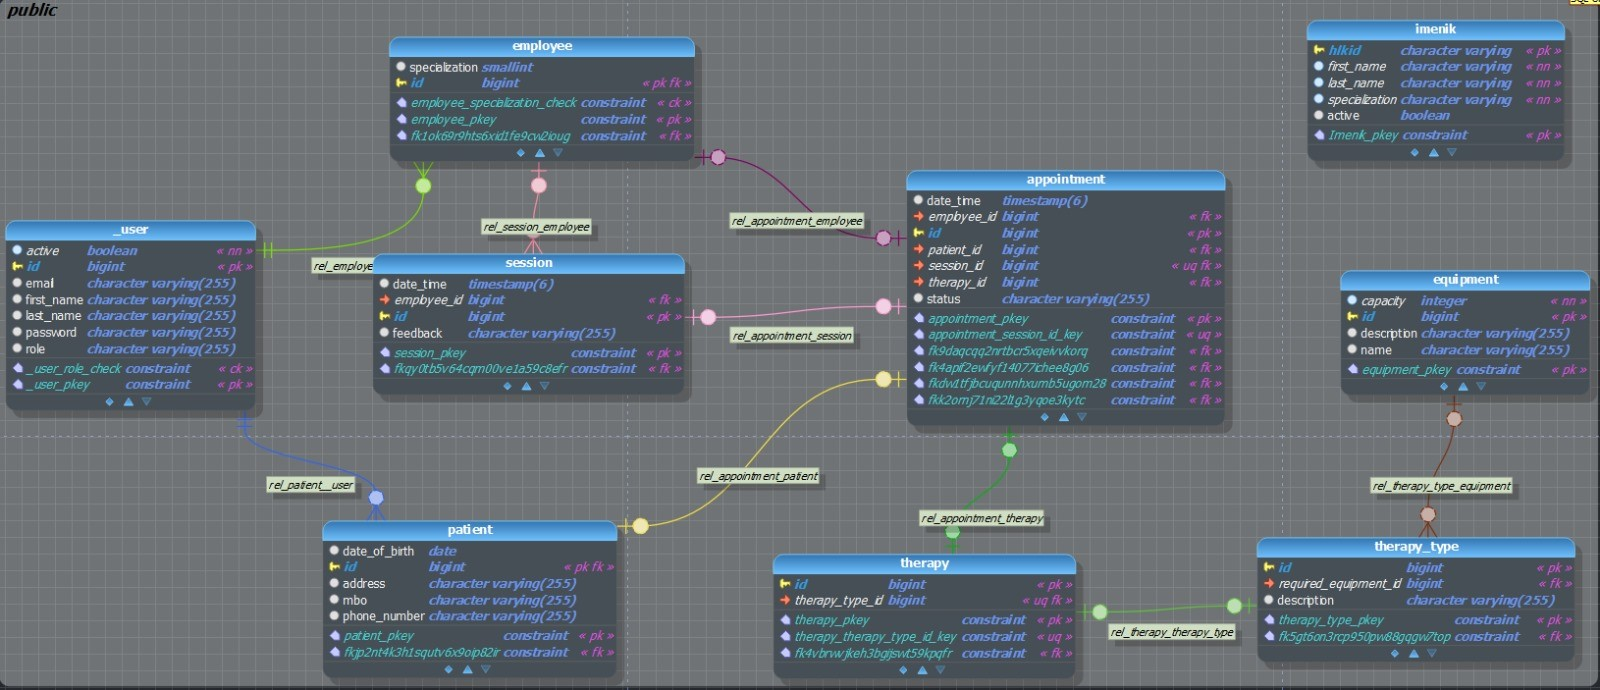
\includegraphics[width=1\linewidth]{slike/database_pr1.jpg}
			    \caption{Dijagram baze podataka}
			    
			    \label{fig:enter-label}
			\end{figure}
			\eject
			
			
		\section{Dijagram razreda}
		
			\textit{Potrebno je priložiti dijagram razreda s pripadajućim opisom. Zbog preglednosti je moguće dijagram razlomiti na više njih, ali moraju biti grupirani prema sličnim razinama apstrakcije i srodnim funkcionalnostima.}\\
			
			\textbf{\textit{dio 1. revizije}}\\
			
			\textit{Prilikom prve predaje projekta, potrebno je priložiti potpuno razrađen dijagram razreda vezan uz \textbf{generičku funkcionalnost} sustava. Ostale funkcionalnosti trebaju biti idejno razrađene u dijagramu sa sljedećim komponentama: nazivi razreda, nazivi metoda i vrste pristupa metodama (npr. javni, zaštićeni), nazivi atributa razreda, veze i odnosi između razreda.}\\
			
			\textbf{\textit{dio 2. revizije}}\\			
			
			\textit{Prilikom druge predaje projekta dijagram razreda i opisi moraju odgovarati stvarnom stanju implementacije}
			
			
			
			\eject
		
		\section{Dijagram stanja}
			
			
			\textbf{\textit{dio 2. revizije}}\\
			
			\textit{Potrebno je priložiti dijagram stanja i opisati ga. Dovoljan je jedan dijagram stanja koji prikazuje \textbf{značajan dio funkcionalnosti} sustava. Na primjer, stanja korisničkog sučelja i tijek korištenja neke ključne funkcionalnosti jesu značajan dio sustava, a registracija i prijava nisu. }
			
			
			\eject 
		
		\section{Dijagram aktivnosti}
			
			\textbf{\textit{dio 2. revizije}}\\
			
			 \textit{Potrebno je priložiti dijagram aktivnosti s pripadajućim opisom. Dijagram aktivnosti treba prikazivati značajan dio sustava.}
			
			\eject
		\section{Dijagram komponenti}
		
			\textbf{\textit{dio 2. revizije}}\\
		
			 \textit{Potrebno je priložiti dijagram komponenti s pripadajućim opisom. Dijagram komponenti treba prikazivati strukturu cijele aplikacije.}
